%%%%%%%%%%%%%%%%%%%%%%%%%%% asme2ej.tex %%%%%%%%%%%%%%%%%%%%%%%%%%%%%%%
% Template for producing ASME-format journal articles using LaTeX    %
% Written by   Harry H. Cheng, Professor and Director                %
%              Integration Engineering Laboratory                    %
%              Department of Mechanical and Aeronautical Engineering %
%              University of California                              %
%              Davis, CA 95616                                       %
%              Tel: (530) 752-5020 (office)                          %
%                   (530) 752-1028 (lab)                             %
%              Fax: (530) 752-4158                                   %
%              Email: hhcheng@ucdavis.edu                            %
%              WWW:   http://iel.ucdavis.edu/people/cheng.html       %
%              May 7, 1994                                           %
% Modified: February 16, 2001 by Harry H. Cheng                      %
% Modified: January  01, 2003 by Geoffrey R. Shiflett                %
% Use at your own risk, send complaints to /dev/null                 %
%%%%%%%%%%%%%%%%%%%%%%%%%%%%%%%%%%%%%%%%%%%%%%%%%%%%%%%%%%%%%%%%%%%%%%

%%% use twocolumn and 10pt options with the asme2ej format
\documentclass[twocolumn,10pt]{asme2ej}

\usepackage{graphicx} %% for loading jpg figures
\usepackage{hyperref}   % to set up hyperlinks
\usepackage{amsmath}
\hypersetup{
	colorlinks=true,
	linkcolor=blue,
	citecolor=blue,
	urlcolor=blue,
}

\usepackage[square,numbers]{natbib}

%% The class has several options
%  onecolumn/twocolumn - format for one or two columns per page
%  10pt/11pt/12pt - use 10, 11, or 12 point font
%  oneside/twoside - format for oneside/twosided printing
%  final/draft - format for final/draft copy
%  cleanfoot - take out copyright info in footer leave page number
%  cleanhead - take out the conference banner on the title page
%  titlepage/notitlepage - put in titlepage or leave out titlepage
%  
%% The default is oneside, onecolumn, 10pt, final


\title{Flow noise estimation models for axial flow past towed
sonar arrays}

%%% first author
\author{Rakesh Sekharipuram Sekar
    \affiliation{
	Student\\
	Department of Mechanical Engineering\\
	Indian Institute of Technology Palakkad\\
	Kanjikode, Palakkad, Kerala, 678623\\
	India\\
    Email: 132203001@smail.iitpkd.ac.in
    }	
}

%%% second author
%%% remove the following entry for single author papers
%%% add more entries for additional authors
\author{Senthil Rajan S
    \affiliation{ Scientist\\
	Naval Physical and Oceanographic Laboratory\\
	Kochi, Kerala, 682021\\
	India\\
        Email: senthilrajan.npol@gov.in
    }
}

%%% third author
%%% remove the following entry for single author papers
%%% add more entries for additional authors
\author{Dr. Anoop Akkoorath Mana\thanks{Address all correspondence related to ASME style format and figures to this author. Address all correspondence for other issues to this author.}
\affiliation{
        Assistant Professor\\
    Department of Mechanical Engineering\\
	Indian Institute of Technology Palakkad\\
	Kanjikode, Palakkad, Kerala, 678623\\
	India\\
    Email: akkoorath@iitpkd.ac.in
    }
}


\begin{document}

\maketitle    

%%%%%%%%%%%%%%%%%%%%%%%%%%%%%%%%%%%%%%%%%%%%%%%%%%%%%%%%%%%%%%%%%%%%%%
\begin{abstract}
{\it Towed sonar arrays house a series of pressure sensors inside a fluid-filled elastic tube. Towing of the sonar array in water generates a turbulent boundary layer on the exterior surface of the elastic tube. The pressure fluctuations in the turbulent boundary layer along with other ambient pressure fluctuations, excites the elastic tube and further generates pressure disturbances in the interior fluid. In this work, a new semi-empirical model of the turbulent pressure spectrum is presented. The new model predictions show a closer agreement with the available experimental results at all tow speeds. A three-dimensional vibroacoustic model of the fluid-filled elastic tube is also presented in this work. The vibroacoustic model is fully coupled and considers both breathing mode and first order variations in the elastic tube and the acoustic field variables. Further, the turbulent pressure spectrum semi-empirical model and the three-dimensional vibroacoustic model are used to compute the on-axis sound pressure level due to the external turbulent pressure excitation at different elastic tube diameters and tow speeds. At low frequencies, increasing tube diameter has little effect on flow noise, while at higher frequencies, flow noise decreases with larger diameters. Increasing tow speed raises flow noise across all frequencies.  
}
\end{abstract}

%%%%%%%%%%%%%%%%%%%%%%%%%%%%%%%%%%%%%%%%%%%%%%%%%%%%%%%%%%%%%%%%%%%%%%
\begin{nomenclature}
\entry{A}{You may include nomenclature here.}
\entry{$\alpha$}{There are two arguments for each entry of the nomemclature environment, the symbol and the definition.}
\end{nomenclature}

The primary text heading is  boldface and flushed left with the left margin.  The spacing between the  text and the heading is two line spaces.

%%%%%%%%%%%%%%%%%%%%%%%%%%%%%%%%%%%%%%%%%%%%%%%%%%%%%%%%%%%%%%%%%%%%%%
\section{Introduction}

Towed sonar arrays contain a series of pressure sensors enclosed within a fluid-filled elastic tube. As the sonar array is towed through the water, a thick layer of turbulent flow is generated over the exterior surface of the tube.~The pressure fluctuations in this turbulent boundary layer (TBL), along with other ambient sea pressure variations, excite the elastic tube and subsequently produce acoustic pressure disturbances within the interior fluid. The hydrophones placed in the interior fluid picks these acoustic signals. The signals associated with the turbulent pressure fluctuations are called flow noise. Currently, the flow noise is measured either by towing the sonar array in open water using a dinghy or by allowing the hydrophone to free fall in water \cite{Sarath2010}. In the first case, noise from the boat and vibrations of the towline connections pollute the measured acoustic signals \cite{Unni2011}; whereas in the second case, the useful measurements can be made only at the terminal velocity of the hydrophone. This work aims at developing a fully coupled vibroacoustic model for predicting the flow noise in towed sonar arrays which is useful over wide range of towing speeds and tube diameters.

%\subsection{Flow over a flat plate}
A widely used model for predicting the turbulent pressure spectrum is that developed by G M Corcos \cite{corcos1963} for the flow over a flat plate. In this model, the turbulent pressure is varying exponentially with respect to both the axes of the flat plate. Although this model is widely used in engineering applications, it has a major shortcoming that it is overestimating the pressure level at low wavenumbers. D M Chase \cite{Chase1981} presented a simpler turbulent pressure spectrum model for the flow over a flat plate. The model is based on experimental observations and uses direct dependence on the flow and dimensional parameters. Frendi et al.~\cite{frendi2020} analysed the Corcos \cite{corcos1963} model and proposed a turbulent model for the flow over a flat plate based on large eddy simulation (LES) and direct numerical simulation (DNS) computational results. Frendi's model involves the use of an auto spectrum which was derived by Michael Goody \cite{goody2004}. The Frendi model predictions are found to match well with an earlier experimental result on flow over a flat plate. Some of the observations of the Chase and Frendi models are relevant to the present work and are discussed in section \ref{sec:empmodels}. Roni Francis et al.~\cite{francis2023} used LES and Reynolds averaged Navier Stokes (RANS) computational method to study the wavenumber frequency spectrum of the turbulent pressure field over a flat plate. This work presents an exhaustive discussion on similar problems in the literature.

% A P Dowling~\cite{Dowling1998} used Lighthill's  theory of aerodynamics to understand under water flow noise. The theory provides a formal way to relate the center-line pressures of an acoustic streamer to the blocked surface pressure spectrum, allowing the effects of the mechanical properties of the streamer to be displayed explicitly. Dowling reviewed the results for a liquid filled streamer and a visco elastic filled streamer, showing that non-zero shear wave speed in the visco elastic medium raises the varicose wave speed. However, the visco elastic-filled streamer's low wave number performance is degraded if there is a small liquid core, causing a noisy low wave number regime.

% According to G. P. Haddle and E. J. Skudrzyk~\cite{Haddle1969}, even at low frequencies, the recorded level of flow noise in water depends on the size and shape of the recording hydrophone rather than the vehicle causing the turbulence.  They also discuss the paradox that, despite numerous theories suggesting that a hydrophone's flow noise sensitivity asymptotically decreases to zero as its size increases, in practice a large hydrophone still picks up flow noise. According to Haddle, the majority of issues in underwater acoustics are caused by a radiation component of flow noise, which calls for additional research.


%\subsection{Axial flow past a cylinder}
D M Chase~\cite{Chase1981} developed a model for computing the turbulent pressure spectrum for an axial flow past a cylinder by modifying his earlier flat plate model. While modifying, Chase considered the radius of the cylinder as one of the parameters instead of the length of the flat plate. Chase derived azimuthal harmonic spectral density by integrating the turbulent pressure spectrum of the flat plate in the cross-flow direction. The details of this model are presented in section \ref{Chase model}. 


A L Carpenter et al.~\cite{carpenter1983} conducted experiments for finding the flow noise inside a fluid-filled elastic tube while towed behind a ship and compared the results with that predicted by  Chase~\cite{Chase1981}. The authors also proposed a tube transfer function for computing the flow noise inside the tube. Andrew Knight~\cite{knight1996} performed similar analytical simulations as in \cite{carpenter1983} but with different types of hydrophones and compared the flow noise with that for an ideal hydrophone. The ideal hydrophone was assumed to have unit acoustic response and zero convective response. This paper also uses an approximate tube transfer function to find the noise inside the fluid-filled elastic tube.\par


Unnikrishnan et al.~\cite{Unni2011} performed experiments to measure the turbulent pressure field outside the elastic tube by towing the sonar array in a quiet lake at different speeds. The work presents a comparison of the experimental results with the available semi-empirical model predictions. It was found that the semi-empirical model estimations match with the measurements only at high tow speeds. Karthik et al.~\cite{karthik2021} studied the turbulent pressure spectrum over a cylinder with the help of an LES computational model. The model predictions match well with the experimental results of Unnikrishnan et al.~\cite{Unni2011}. Karthik et al. also presented a non-dimensional turbulent flow noise spectrum for easy estimation of the spectrum at different tow speeds and tube diameters.

Both Carpenter et al.\cite{carpenter1983} and Andrew Knight~\cite{knight1996} estimated the flow noise inside a fluid-filled elastic tube with the help of the Chase model for the turbulent pressure spectrum and an approximate tube transfer function. Jineesh et al.~\cite{jineesh2013} developed a better axisymmetric model of the fluid-filled elastic tube and used it to estimate the flow noise inside the tube. It was found that the earlier approximate transfer function model overestimates the flow noise inside the tube.

This paper develops a new semi-empirical model for the turbulent pressure spectrum of axial flow past a solid cylinder. It also presents a fully coupled three-dimensional vibroacoustic model of a fluid-filled elastic tube. Furthermore, these models are used to compute the on-axis sound pressure level resulting from external turbulent pressure excitation on the elastic tube. The organization of the paper is as follows: Section.~\ref{sec:empmodels} discusses two existing semi-empirical models for estimating turbulent pressure spectrum for axial flow past a solid cylinder. Section.~\ref{sec:hybmodel} discusses the development of a new semi-empirical model for the turbulent pressure spectrum, which provides improved predictions compared to existing models. Section.~\ref{sec:vamodel} discusses the development of a three-dimensional vibroacoustic model to estimate the on-axis flow noise inside a fluid-filled elastic tube. Further, Section.~\ref{sec:results} discusses the estimation of interior acoustic pressure spectrum and on-axis flow noise inside a fluid-filled elastic tube and are compared with the existing results.


\section{Review of semi-empirical models of turbulent pressure spectrum} \label{sec:empmodels}
One of the aim of this study is to predict the flow noise resulting from turbulent boundary layer excitation. To achieve this, a semi-empirical model that can estimate the turbulent pressure exerted by fluid flow on a cylindrical tube, is required. Two existing semi-empirical models for turbulent pressure fluctuation is discussed in this section. Furthermore, flow noise at the outer surface of the solid cylinder is estimated using these models, showing its variation in comparison to available experimental results~\cite{Unni2011}. 
%\label{pressure spectrum}

\subsection{Chase model}\label{Chase model}
Chase~\cite{Chase1981} proposed a semi-empirical model for predicting the frequency-wavenumber spectrum of turbulent pressure field over a solid cylinder and is given by
\begin{multline}
        \hat{p}_{0}(k_{z},\omega) = C\rho^{2}\nu_{*}^{3}R^2\biggl[(k_{z}R)^{2}+\frac{1}{12}\biggr]\\ \biggl[\frac{(\omega R-u_{c}k_{z}R)^{2}}{h^{2}\nu_{*}^{2}}+(k_{z}R)^{2}+b_1^{-2}\biggr]^{-2.5}.
		\label{Turbulent pressure spectrum equation Chase}
\end{multline}


%%%%%%%%%%%%%%%%%%%%%%%%%%%%%%%%%%%%%%%%%%%%%%%%%%%%%%%%%%%%%%%%%%%%%%
\section{Very Very Very Very Very Very Very Very Very Very Very Long Heading}

The heading is boldface with upper and lower case letters. 
If the heading should run into more than one line, the run-over is not left-flushed.

%%%%%%%%%%%%%%%%%%%%%%%%%%%%%%%%%%%%%%%%%%%%%%%%%%%%%%%%%%%%%%%%%%%%%%
\subsection{Second-Level Heading}

The next level of heading is also boldface with upper and lower case letters. 
The heading is flushed left with the left margin. The spacing to the next heading is two line spaces.

%%%%%%%%%%%%%%%%%%%%%%%%%%%%%%%%%%%%%%%%%%%%%%%%%%%%%%%%%%%%%%%%%%%%%%
\subsubsection{Third-Level Heading.}

The third-level of heading follows the style of the second-level heading.


%%%%%%%%%%%%%%%%%%%%%%%%%%%%%%%%%%%%%%%%%%%%%%%%%%%%%%%%%%%%%%%%%%%%%%
\section{Use of SI Units}

An ASME paper should use SI units.  When preference is given to SI units, the U.S. customary units may be given in parentheses or omitted. When U.S. customary units are given preference, the SI equivalent {\em shall} be provided in parentheses or in a supplementary table. 

%%%%%%%%%%%%%%%%%%%%%%%%%%%%%%%%%%%%%%%%%%%%%%%%%%%%%%%%%%%%%%%%%%%%%%
\section{Footnotes\protect\footnotemark}
\footnotetext{Examine the input file, asme2ej.tex, to see how a footnote is given in a head.}

Footnotes are referenced with superscript numerals and are numbered consecutively from 1 to the end of the paper\footnote{Avoid footnotes if at all possible.}. Footnotes should appear at the bottom of the column in which they are referenced.


%%%%%%%%%%%%%%%%%%%%%%%%%%%%%%%%%%%%%%%%%%%%%%%%%%%%%%%%%%%%%%%%%%%%%%
\section{Mathematics}

Equations should be numbered consecutively beginning with (1) to the end of the paper, including any appendices.  The number should be enclosed in parentheses and set flush right in the column on the same line as the equation.  An extra line of space should be left above and below a displayed equation or formula. \LaTeX\ can automatically keep track of equation numbers in the paper and format almost any equation imaginable. An example is shown in Eqn.~(\ref{eq_ASME}). The number of a referenced equation in the text should be preceded by Eqn.\ unless the reference starts a sentence in which case Eqn.\ should be expanded to Equation.

\begin{equation}
f(t) = \int_{0_+}^t F(t) dt + \frac{d g(t)}{d t}
\label{eq_ASME}
\end{equation}

%%%%%%%%%%%%%%%%%%%%%%%%%%%%%%%%%%%%%%%%%%%%%%%%%%%%%%%%%%%%%%%%%%%%%%
\section{Figures}
\label{sect_figure}

All figures should be positioned at the top of the page where possible.  All figures should be numbered consecutively and centered under the figure as shown in Fig.~\ref{figure_ASME}. All text within the figure should be no smaller than 7~pt. There should be a minimum two line spaces between figures and text. The number of a referenced figure or table in the text should be preceded by Fig.\ or Tab.\ respectively unless the reference starts a sentence in which case Fig.\ or Tab.\ should be expanded to Figure or Table.


%%%%%%%%%%%%%%%%%%%%%%%%%%%%%%%%%%%%%%%%%%%%%%%%%%%%%%%%%%%%%%%%%%%%%%
%%%%%%%%%%%%%%%% begin figure %%%%%%%%%%%%%%%%%%%
\begin{figure}[t]
\begin{center}
\setlength{\unitlength}{0.012500in}%
\begin{picture}(115,35)(255,545)
\thicklines
\put(255,545){\framebox(115,35){}}
\put(275,560){Beautiful Figure}
\end{picture}
\end{center}
\caption{The caption of a single sentence does not have period at the end}
\label{figure_ASME} 
\end{figure}
%%%%%%%%%%%%%%%% end figure %%%%%%%%%%%%%%%%%%% 
%%%%%%%%%%%%%%%%%%%%%%%%%%%%%%%%%%%%%%%%%%%%%%%%%%%%%%%%%%%%%%%%%%%%%%

In the following subsections, I have inserted figures that have been provided by authors in order to demonstrate what to avoid.  In each case the authors provided figures that are 3.25in wide and 600dpi in the .tif graphics format.  The papers containing these figures have been held from production due to their poor quality. 

%%%%%%%%%%%%%%%%%%%%%%%%%%%%%%%%%%%%%%%%%%%%%%%%%%%%%%%%%%%%%%%%%%%%%%
\subsection{The 1st Example of Bad Figure}

%%%%%%%%%%%%%%%% begin figure %%%%%%%%%%%%%%%%%%%
%%% 3.34in is the maximum width you can have for a figure
\begin{figure} 
\centerline{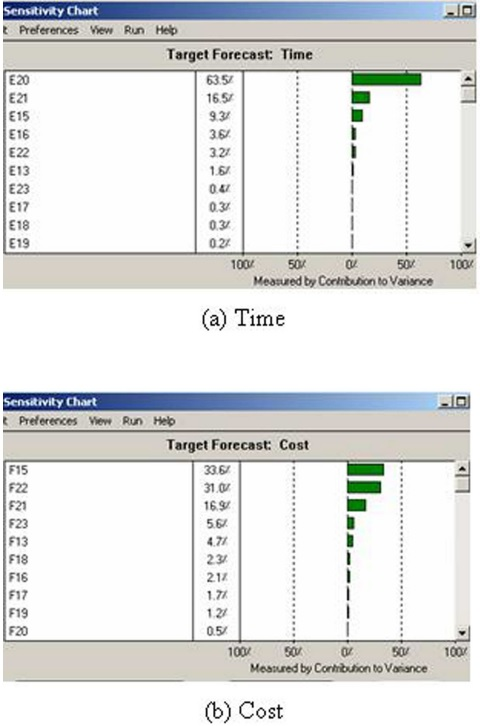
\includegraphics[width=3.34in]{figure/FMANU_MD_05_1107_11.jpg}}
\caption{Example taken from a paper that was held from production because the image quality is poor.  ASME sets figures captions in 8pt, Helvetica Bold.}
\label{fig_example1.jpg}
\end{figure}
%%%%%%%%%%%%%%%% end figure %%%%%%%%%%%%%%%%%%%

In order to place the figure in this template using MSWord, select Insert Picture from File, and use wrapping that is top and bottom. Make sure the figure is 3.25in wide.
 
Figure~`\ref{fig_example1.jpg}
was taken from a recent paper that was held from publication, because the text is fuzzy and unreadable. It was probably obtained by taking a screen shot of the computer output of the authors software. This means the original figure was 72dpi (dots per inch) on a computer screen. There is no way to improve the quality such a low resolution figure.
 
In order to understand how poor the quality of this figure is, please zoom in slightly, say to 200\%.  Notice that while the font of the paper is clear at this size, the font in the figures is fuzzy and blurred.  It is impossible to make out the small symbol beside the numbers along the abscissa of the graph.  Now consider the labels Time and Cost. They are clearly in fonts larger that the text of the article, yet the pixilation or rasterization, associated with low resolution is obvious. This figure must be regenerated at higher resolution to ensure quality presentation.

The poor quality of this figure is immediately obvious on the printed page, and reduces the impact of the research contribution of the paper, and in fact detracts from the perceived quality of the journal itself.



%%%%%%%%%%%%%%%%%%%%%%%%%%%%%%%%%%%%%%%%%%%%%%%%%%%%%%%%%%%%%%%%%%%%%%
\subsection{The 2nd Example of Bad Figure}

%%%%%%%%%%%%%%%% begin figure %%%%%%%%%%%%%%%%%%%
\begin{figure} 
\centerline{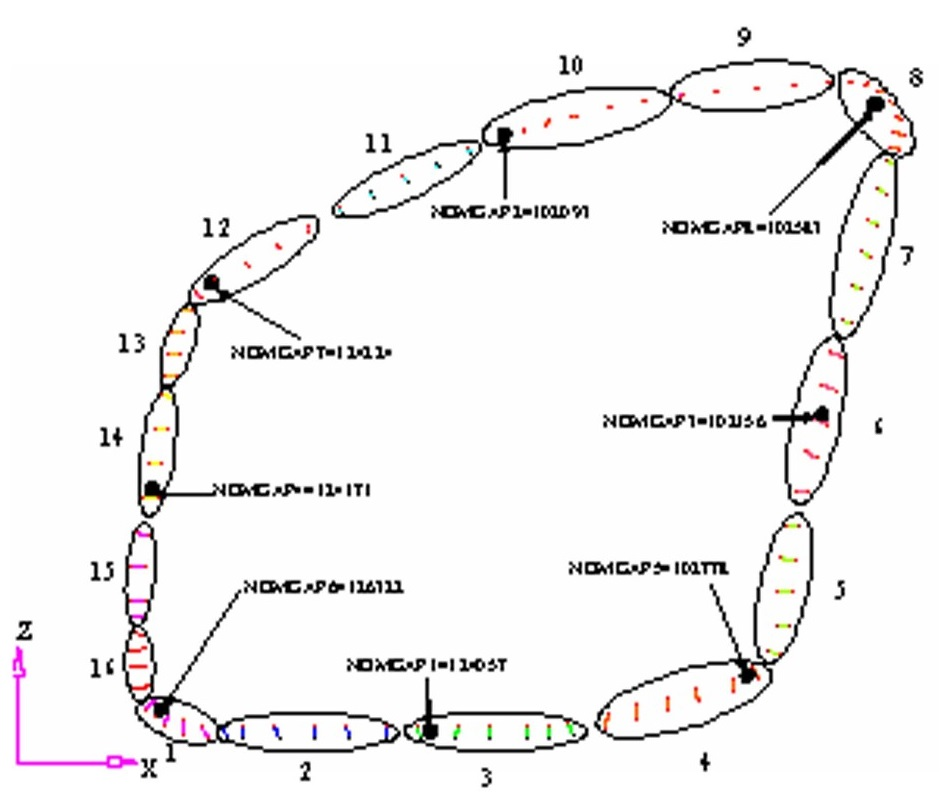
\includegraphics[width=3.34in]{figure/FMANU_MD_05_1272_5.jpg}}
\caption{While this figures is easily readable at a double column width of 6.5in, when it is shrunk to 3.25in column width the text is unreadable. This paper was held from production.}
\label{fig_example2.jpg}
\end{figure}
%%%%%%%%%%%%%%%% end figure %%%%%%%%%%%%%%%%%%%

Figure~\ref{fig_example2.jpg}
demonstrates a common problem that arises when a figure is scaled down fit a single column width of 3.25in.  The original figure had labels that were readable at full size, but become unreadable when scaled to half size.  This figure also suffers from poor resolution as is seen in the jagged lines the ovals that form the chain.

This problem can be addressed by increasing the size of the figure to a double column width of 6.5in, so the text is readable.  But this will not improve the line pixilation, and a large low resolution figure is less desirable than a small one.  This also significantly expands the length of the paper, and may cause it to exceed the JMD nine page limit.  Additional pages require page charges of \$200 per page.  It is best to regenerate the figure at the resolution that ensures a quality presentation.


%%%%%%%%%%%%%%%%%%%%%%%%%%%%%%%%%%%%%%%%%%%%%%%%%%%%%%%%%%%%%%%%%%%%%%
\subsection{The 3rd Example of Bad Figure}
%%%%%%%%%%%%%%%% begin figure %%%%%%%%%%%%%%%%%%%
\begin{figure} 
\centerline{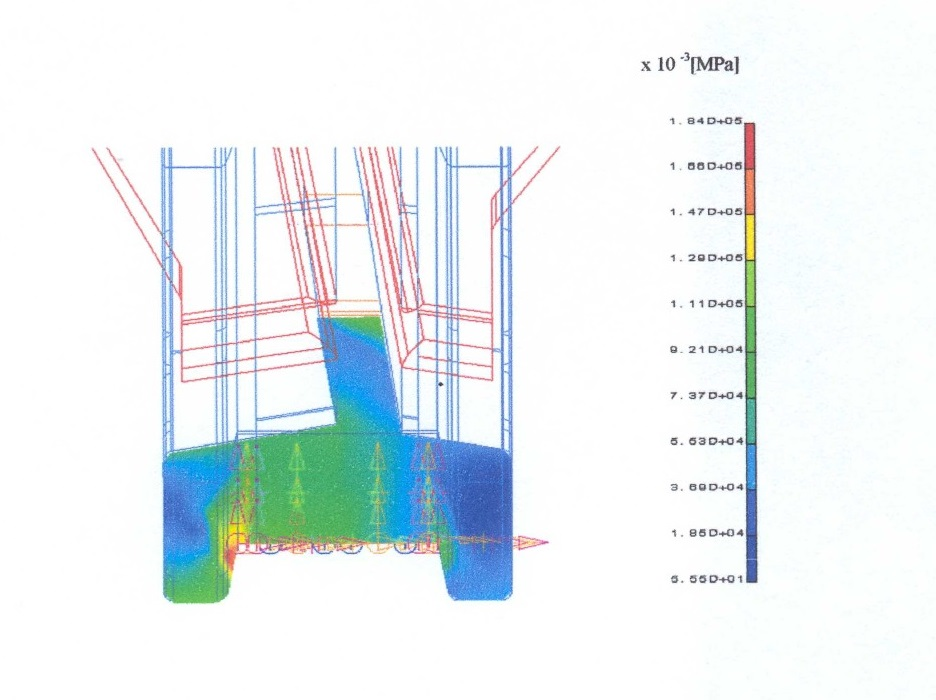
\includegraphics[width=3.25in]{figure/FMANU_MD_04_1274_13.jpg}}
\caption{Another example of a figure with unreadable text.  Even when the paper was expanded to double column width the text as shown in Fig.~\ref{fig_example4.jpg} was of such low quality that the paper was held from production.}
\label{fig_example3.jpg}
\end{figure}
%%%%%%%%%%%%%%%% end figure %%%%%%%%%%%%%%%%%%%

%%%%%%%%%%%%%%%% begin figure %%%%%%%%%%%%%%%%%%%
%%% the maximum width in double column is 6.85in
\begin{figure*} 
\centerline{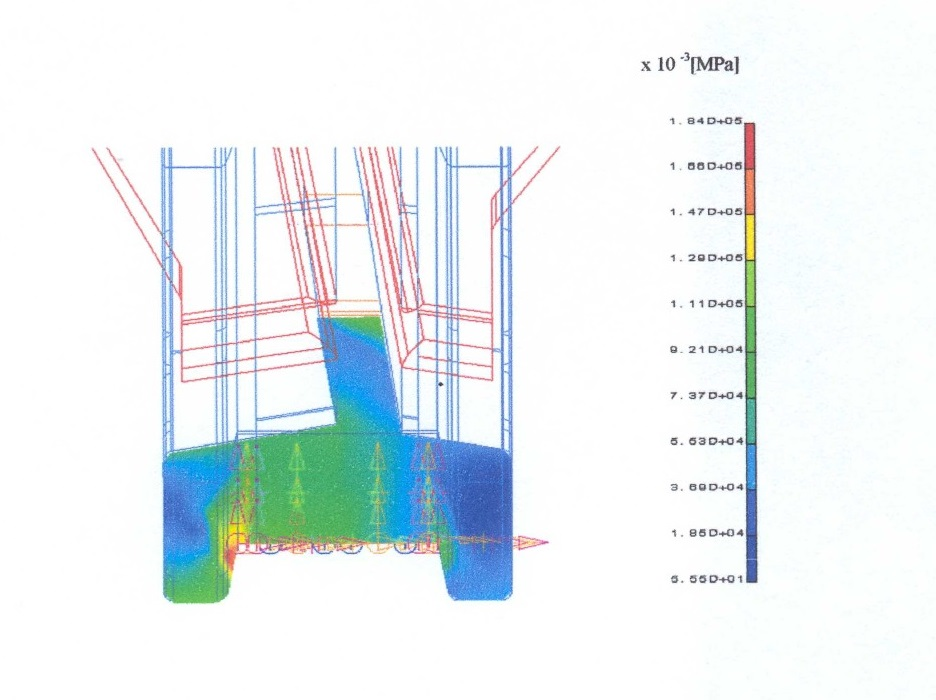
\includegraphics[width=6.85in]{figure/FMANU_MD_04_1274_13.jpg}}
\caption{A figure expanded to double column width the text from Figure~\ref{fig_example3.jpg}}
\label{fig_example4.jpg}
\end{figure*}
%%%%%%%%%%%%%%%% end figure %%%%%%%%%%%%%%%%%%%
An author provided the high resolution image 
in Fig.~\ref{fig_example3.jpg}
that was sized to a single column width of 3.25in.  Upon seeing the poor quality of the text, the publisher scaled the image to double column width as shown in Fig.~\ref{fig_example4.jpg} 
at which point it took half of a page.  The publisher went on to do this for all eight figures generating four pages of figures that the author did not expect. ASME stopped production of the paper even with the larger figures due to the pixilation of the font.

Clearly the text in this figure is unreadable, and it is doubtful that the author can print the output in a way that it is readable.  This is a problem that the author must solve, not the publisher. 

As you might expect, I have many more examples, but in the end the author is the best judge of what is needed in each figure.  ASME simply requires that the image meet a minimum standard for font and line quality, specifically the font should be the appropriate size and not be blurred or pixilated, and that lines should be the appropriate weight and have minimal, preferably no, pixilation or rasterization.


%%%%%%%%%%%%%%%%%%%%%%%%%%%%%%%%%%%%%%%%%%%%%%%%%%%%%%%%%%%%%%%%%%%%%%
\section{Tables}

%%%%%%%%%%%%%%%%%%%%%%%%%%%%%%%%%%%%%%%%%%%%%%%%%%%%%%%%%%%%%%%%%%%%%%
%%%%%%%%%%%%%%% begin table   %%%%%%%%%%%%%%%%%%%%%%%%%%
\begin{table}[t]
\caption{Figure and table captions do not end with a period}
\begin{center}
\label{table_ASME}
\begin{tabular}{c l l}
& & \\ % put some space after the caption
\hline
Example & Time & Cost \\
\hline
1 & 12.5 & \$1,000 \\
2 & 24 & \$2,000 \\
\hline
\end{tabular}
\end{center}
\end{table}
%%%%%%%%%%%%%%%% end table %%%%%%%%%%%%%%%%%%% 
%%%%%%%%%%%%%%%%%%%%%%%%%%%%%%%%%%%%%%%%%%%%%%%%%%%%%%%%%%%%%%%%%%%%%%

All tables should be numbered consecutively  and centered above the table as shown in Table~\ref{table_ASME}. The body of the table should be no smaller than 7 pt.  There should be a minimum two line spaces between tables and text.


%%%%%%%%%%%%%%%%%%%%%%%%%%%%%%%%%%%%%%%%%%%%%%%%%%%%%%%%%%%%%%%%%%%%%%
\section{Citing References}

%%%%%%%%%%%%%%%%%%%%%%%%%%%%%%%%%%%%%%%%%%%%%%%%%%%%%%%%%%%%%%%%%%%%%%
The ASME reference format is defined in the authors kit provided by the ASME.  The format is:

\begin{quotation}
{\em Text Citation}. Within the text, references should be cited in  numerical order according to their order of appearance.  The numbered reference citation should be enclosed in brackets.
\end{quotation}

The references must appear in the paper in the order that they were cited.  In addition, multiple citations (3 or more in the same brackets) must appear as a `` [1-3]''.  A complete definition of the ASME reference format can be found in the  ASME manual \cite{asmemanual}.

The bibliography style required by the ASME is unsorted with entries appearing in the order in which the citations appear. If that were the only specification, the standard {\sc Bib}\TeX\ unsrt bibliography style could be used. Unfortunately, the bibliography style required by the ASME has additional requirements (last name followed by first name, periodical volume in boldface, periodical number inside parentheses, etc.) that are not part of the unsrt style. Therefore, to get ASME bibliography formatting, you must use the \verb+asmems4.bst+ bibliography style file with {\sc Bib}\TeX. This file is not part of the standard BibTeX distribution so you'll need to place the file someplace where LaTeX can find it (one possibility is in the same location as the file being typeset).

With \LaTeX/{\sc Bib}\TeX, \LaTeX\ uses the citation format set by the class file and writes the citation information into the .aux file associated with the \LaTeX\ source. {\sc Bib}\TeX\ reads the .aux file and matches the citations to the entries in the bibliographic data base file specified in the \LaTeX\ source file by the \verb+\bibliography+ command. {\sc Bib}\TeX\ then writes the bibliography in accordance with the rules in the bibliography .bst style file to a .bbl file which \LaTeX\ merges with the source text.  A good description of the use of {\sc Bib}\TeX\ can be found in \cite{latex, goosens} (see how two references are handled?).  The following is an example of how three or more references \cite{latex, asmemanual,  goosens} show up using the \verb+asmems4.bst+ bibliography style file in conjunction with the \verb+asme2ej.cls+ class file. Here are some more \cite{art, blt, ibk, icn, ips, mts, mis, pro, pts, trt, upd} which can be used to describe almost any sort of reference.

%%%%%%%%%%%%%%%%%%%%%%%%%%%%%%%%%%%%%%%%%%%%%%%%%%%%%%%%%%%%%%%%%%%%%%
\section{Conclusions}
The only way to ensure that your figures are presented in the ASME Journal of Mechanical Design in the way you feel is appropriate and meets the requirement for quality presentation is for you to prepare a double column version of the paper in a form similar to that used by the Journal.

This gives you the opportunity to ensure that the figures are sized appropriately, in particular that the labels are readable and match the size of the text in the journal, and that the line weights and resolutions have no pixilation or rasterization.  Poor quality figures are immediately obvious on the printed page, and this detracts from the perceived quality of the journal.

I am pleased to provide advice on how to improve any figure, but this effort must start with a two-column version of the manuscript. Thank you in advance for your patience with this effort, it will ensure quality presentation of your research contributions.



%%%%%%%%%%%%%%%%%%%%%%%%%%%%%%%%%%%%%%%%%%%%%%%%%%%%%%%%%%%%%%%%%%%%%%
\section{Discussions}
This template is not yet ASME journal paper format compliant at this point.
More specifically, the following features are not ASME format compliant.
\begin{enumerate}
\item
The format for the title, author, and abstract in the cover page.
\item
The font for title should be 24 pt Helvetica bold.
\end{enumerate}

\noindent
If you can help to fix these problems, please send us an updated template.
If you know there is any other non-compliant item, please let us know.
We will add it to the above list.
With your help, we shall make this template 
compliant to the ASME journal paper format.


%%%%%%%%%%%%%%%%%%%%%%%%%%%%%%%%%%%%%%%%%%%%%%%%%%%%%%%%%%%%%%%%%%%%%%
\begin{acknowledgment}
ASME Technical Publications provided the format specifications for the Journal of Mechanical Design, though they are not easy to reproduce.  It is their commitment to ensuring quality figures in every issue of JMD that motivates this effort to have authors review the presentation of their figures.  

Thanks go to D. E. Knuth and L. Lamport for developing the wonderful word processing software packages \TeX\ and \LaTeX. We would like to thank Ken Sprott, Kirk van Katwyk, and Matt Campbell for fixing bugs in the ASME style file \verb+asme2ej.cls+, and Geoff Shiflett for creating 
ASME bibliography stype file \verb+asmems4.bst+.
\end{acknowledgment}

%%%%%%%%%%%%%%%%%%%%%%%%%%%%%%%%%%%%%%%%%%%%%%%%%%%%%%%%%%%%%%%%%%%%%%
% The bibliography is stored in an external database file
% in the BibTeX format (file_name.bib).  The bibliography is
% created by the following command and it will appear in this
% position in the document. You may, of course, create your
% own bibliography by using thebibliography environment as in
%
% \begin{thebibliography}{12}
% ...
% \bibitem{itemreference} D. E. Knudsen.
% {\em 1966 World Bnus Almanac.}
% {Permafrost Press, Novosibirsk.}
% ...
% \end{thebibliography}

% Here's where you specify the bibliography style file.
% The full file name for the bibliography style file 
% used for an ASME paper is asmems4.bst.
\bibliographystyle{asmems4}

% Here's where you specify the bibliography database file.
% The full file name of the bibliography database for this
% article is asme2e.bib. The name for your database is up
% to you.
\bibliography{asme2e}

%%%%%%%%%%%%%%%%%%%%%%%%%%%%%%%%%%%%%%%%%%%%%%%%%%%%%%%%%%%%%%%%%%%%%%
\appendix       %%% starting appendix
\section*{Appendix A: Head of First Appendix}
Avoid Appendices if possible.

%%%%%%%%%%%%%%%%%%%%%%%%%%%%%%%%%%%%%%%%%%%%%%%%%%%%%%%%%%%%%%%%%%%%%%
\section*{Appendix B: Head of Second Appendix}
\subsection*{Subsection head in appendix}
The equation counter is not reset in an appendix and the numbers will
follow one continual sequence from the beginning of the article to the very end as shown in the following example.
\begin{equation}
a = b + c.
\end{equation}

\end{document}
